Так же в третьей главе рассматривается параметрический метод оценки частоты на основе авторегрессионной (АР) - модели сигнала.

Удобство применения АР для задачи оценки частоты обусловлено тем, что в сигнале с расширенным спектром после демодуляции ПСП остается одна
гармоническая компонента и шум (\ref{eq:cdma_strip_eq}).  Даже если входной сигнал содержал другие гармонические компоненты,
после повторной модуляции ПСП они будут "размазаны" по спектру.

Для обнаружения одного гармонического сигнала на фоне аддитивной помехи в виде белого шума достаточно использовать АР модель второго порядка.

Но на качество оценки частоты сильное влияние оказывает точность оценки АКФ. Получение требуемой точности оценки частоты, удовлетворяющей допустимой начальной
расстройке на входе модуля ФАПЧ, возможно только при относительно высоком ОСШ. Для использования данного подхода при низких ОСШ необходимо произвести
увеличение ОСШ.

Увеличение ОСШ с помощью предлагаемого усовершенствованного итеративного алгоритма оценки АКФ, позволяет достичь заданной точности при ОСШ -25 дБ, в то
время как без увеличения ОСШ заданная точность может быть достигнута только при уровне 10 дБ - рисунок \ref{pic:ACF_boost}.

\begin{figure}[H]
\center\scalebox{1}{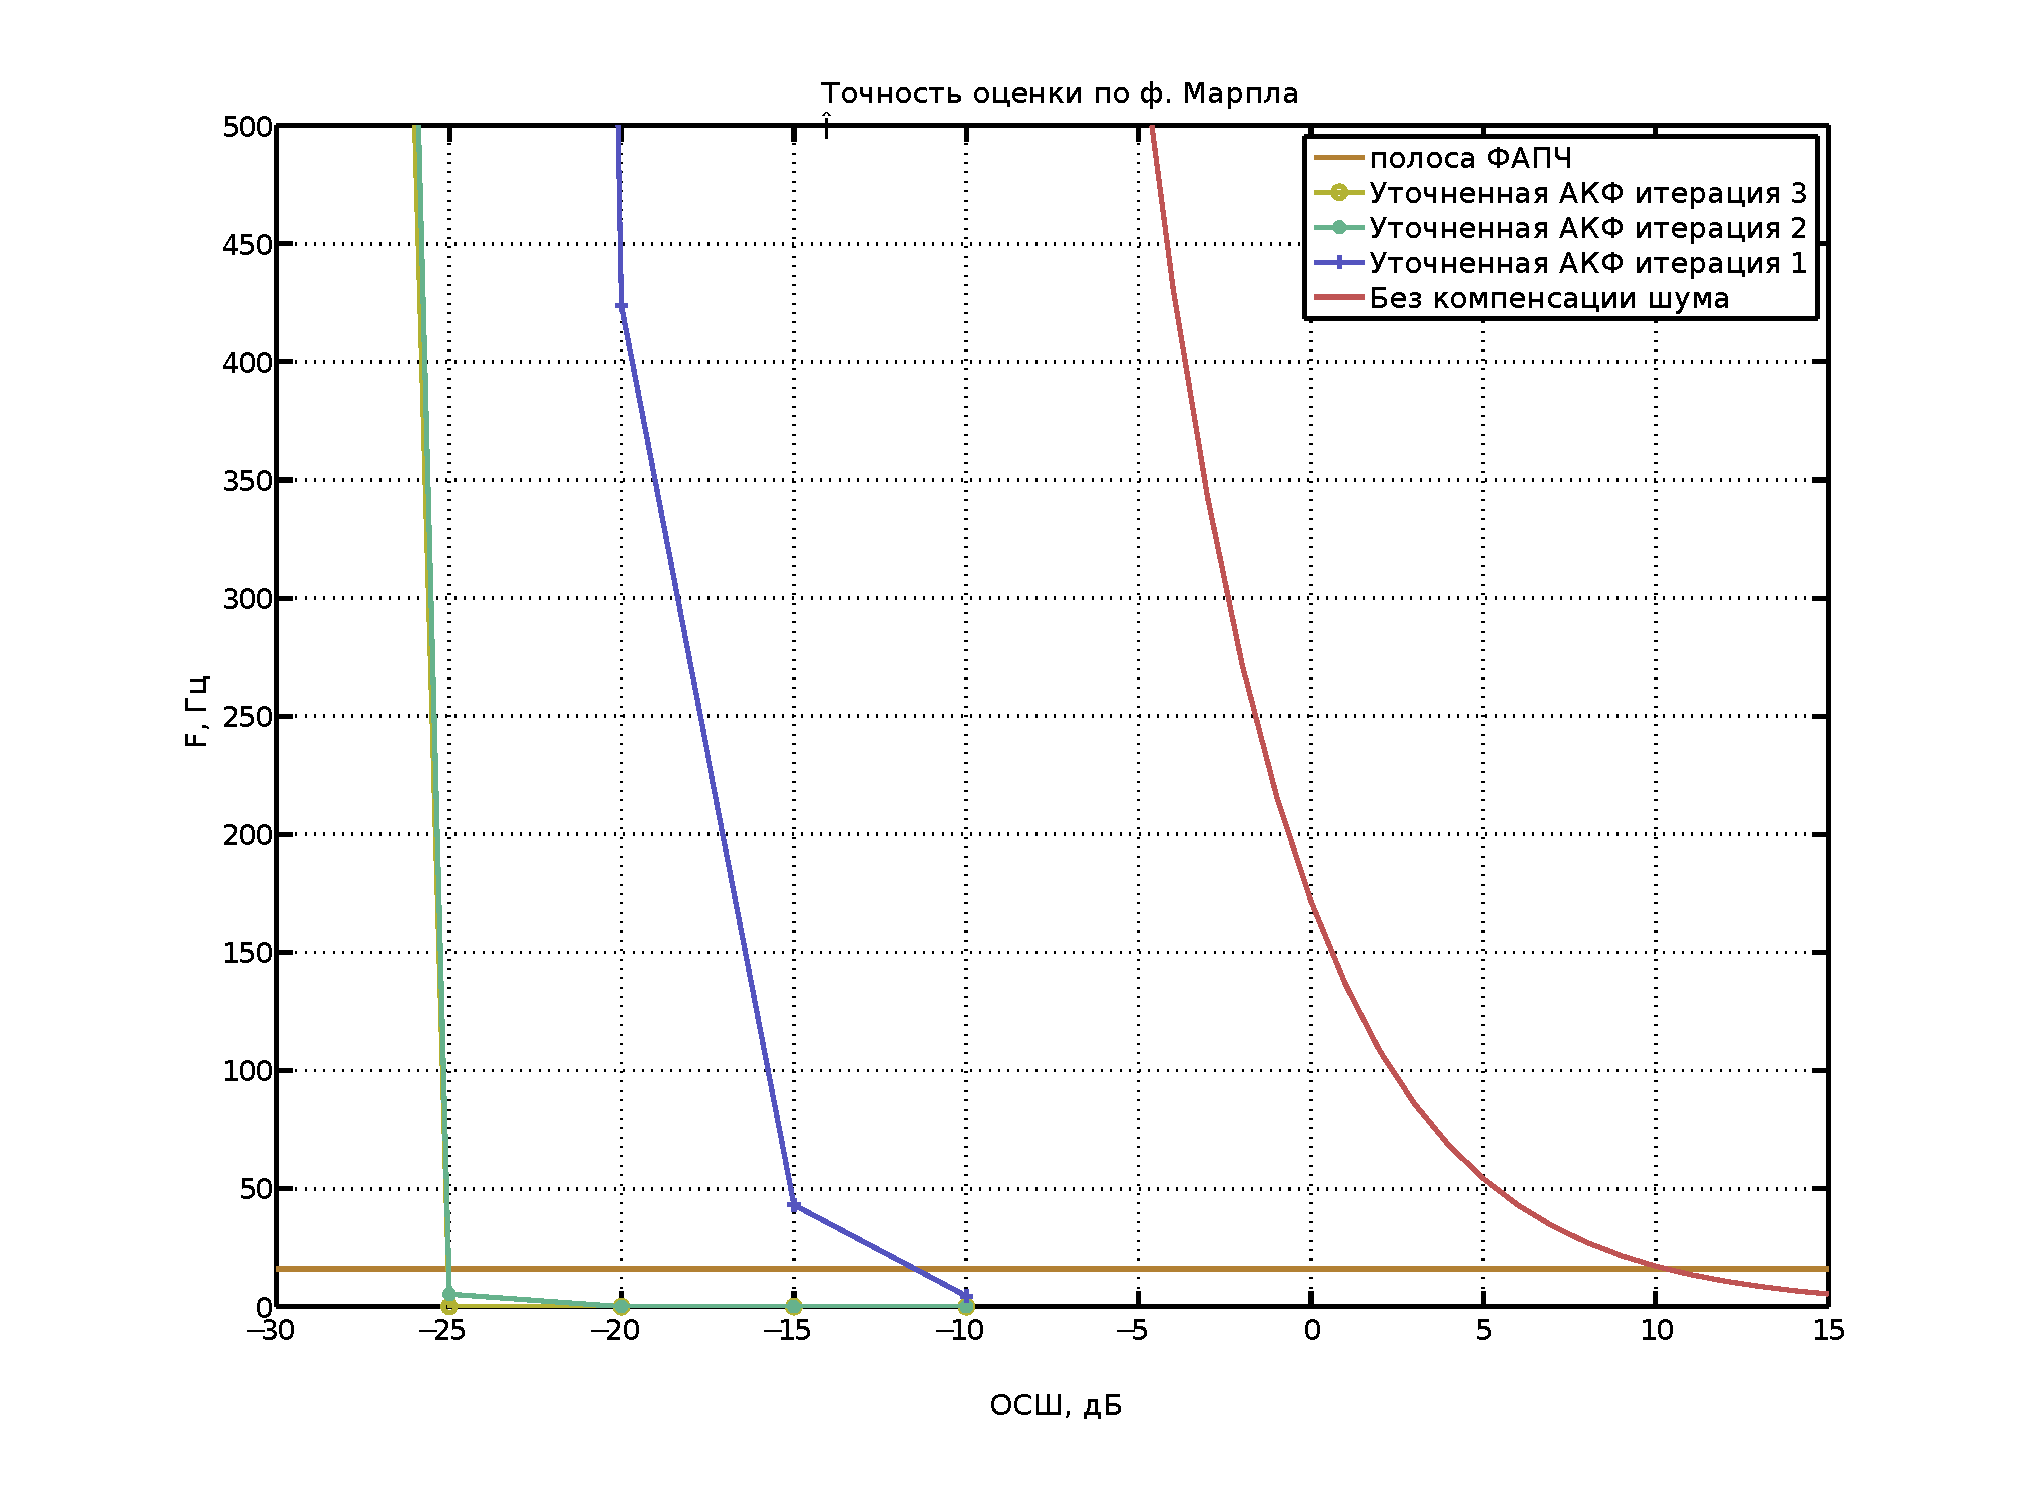
\includegraphics[width=1\linewidth]{ACF_boost.eps}}
	\caption{Точность оценки частоты с компенсацией и без компенсации шума}
	\label{pic:ACF_boost}
\end{figure}
